\chapter{Effect Sizes, Multiple Testing and Pitfalls}
\label{ch:pitfalls}

Chapters 9 and 10 built the machinery: a test statistic, a p-value, a decision.
This chapter is about what goes wrong when that machinery meets real people with
real deadlines. Every tool here has the same aim. You start with a claim that
some result is ``significant'' and work out whether you should actually believe
it, and whether it matters.

\section{Statistical versus practical significance}
\label{sec:pitfalls-practical}

Start with an A/B test on a checkout page. Each arm gets one million visitors.

\begin{center}
\begin{tabular}{lrrr}
\toprule
Arm & Visitors & Purchases & Conversion \\
\midrule
Control $A$ & 1{,}000{,}000 & 100{,}000 & 10.00\% \\
Treatment $B$ & 1{,}000{,}000 & 101{,}000 & 10.10\% \\
\bottomrule
\end{tabular}
\end{center}

The two-proportion $z$-test from Chapter 10 uses the pooled rate
$\hat p = 0.1005$:
\[
  \SE = \sqrt{\hat p(1-\hat p)\left(\tfrac{1}{n_A}+\tfrac{1}{n_B}\right)}
      = \sqrt{0.1005\cdot 0.8995\cdot 2\times 10^{-6}} \approx 0.000425,
\]
\[
  z = \frac{0.1010-0.1000}{0.000425} \approx 2.35,
  \qquad p \approx 0.019 .
\]
The result is ``significant at the 5\% level''. The 95\% confidence interval for
the difference is $0.10 \pm 0.08$ percentage points, roughly $[0.02,\ 0.18]$.
The new page lifts conversion by about one tenth of a percentage point. If the
redesign cost three engineer-months and slows the page, nobody should ship it.

The p-value answered one narrow question: is the difference exactly zero? With a
million users per arm, almost nothing is exactly zero, so almost everything is
``significant''. Here the p-value tells you far more about how big the sample was
than about how big the effect is.

\begin{definition}[Statistical and practical significance]
A result is \textbf{statistically significant} if its p-value falls below the
chosen level $\alpha$: the data are hard to explain by chance alone under the null.
It is \textbf{practically significant} if the size of the effect is large enough to
change a decision. The two are separate questions, and sample size drives the
first much more than the second.
\end{definition}

Figure~\ref{fig:pitfalls-pvsn} holds the true effect fixed at $+0.1$ percentage
points and lets $n$ grow. The p-value you would typically see slides from
$0.94$ to below $10^{-6}$. Nothing about the product changed.

\begin{figure}[H]
\centering
\begin{tikzpicture}
\begin{axis}[
  width=11.5cm, height=6cm,
  xmode=log, xmin=1000, xmax=5000000,
  ymin=0, ymax=1.02,
  xlabel={visitors per arm, $n$},
  ylabel={typical p-value},
  axis lines=left, grid=major, grid style={gray!20},
  title={Same tiny effect ($10.0\%\to10.1\%$), growing sample},
  title style={font=\small},
]
\addplot[distblue, very thick, smooth] coordinates {
(1000,0.9407) (1467.8,0.9282) (2154.4,0.9131) (3162.3,0.8948) (4641.6,0.8727)
(6812.9,0.8461) (10000,0.8141) (14678,0.7757) (21544,0.7299) (31623,0.6758)
(46416,0.6124) (68129,0.5393) (100000,0.4571) (146780,0.3676) (215443,0.275)
(316228,0.186) (464159,0.1091) (681292,0.05224) (1000000,0.01868)
(1467799,0.004382) (2154435,0.0005565) (3162278,0.00002887) (4641589,0.0000004)
};
\draw[trapred, dashed, thick] (axis cs:1000,0.05) -- (axis cs:5000000,0.05);
\node[trapred, anchor=south west, font=\small] at (axis cs:1100,0.06) {$\alpha=0.05$};
\fill[trapred] (axis cs:1000000,0.01868) circle (2.2pt);
\draw[gray] (axis cs:950000,0.025) -- (axis cs:150000,0.2);
\node[anchor=east, font=\small, fill=white, inner sep=1pt] at (axis cs:150000,0.2) {our test: $p=0.019$};
\end{axis}
\end{tikzpicture}
\caption{The p-value computed at the expected $z$ for a fixed lift of $0.1$
percentage points. Grow $n$ and the curve dives under $0.05$ while the effect
stays exactly as small. A small p-value tells you the effect is probably not zero.
It does not tell you the effect is large.}
\label{fig:pitfalls-pvsn}
\end{figure}

The fix is to decide in advance what size of effect would matter. Call it the
\textbf{smallest effect of interest}: the lift below which you would not act,
whatever the p-value. Then read the confidence interval against that threshold.
Figure~\ref{fig:pitfalls-zones} shows the four cases you will meet.

\begin{figure}[H]
\centering
\begin{tikzpicture}[x=1.9cm, y=0.9cm]
\fill[gray!15] (-0.5,0.4) rectangle (0.5,4.6);
\node[font=\small, gray!40!black, align=center] at (0,4.95) {too small\\[-2pt]to matter};
\draw[-{Stealth}] (-2.1,0.4) -- (3.6,0.4);
\foreach \x in {-2,-1,0,1,2,3} {
  \draw (\x,0.32) -- (\x,0.48);
  \node[below, font=\small] at (\x,0.32) {$\x$};
}
\node[below, font=\small] at (0.75,-0.15) {lift in percentage points};
\draw[gray, dashed] (0,0.4) -- (0,4.6);
\draw[targetgreen, very thick, |-|] (1.2,4) -- (3.0,4);
\fill[targetgreen] (2.1,4) circle (2.5pt);
\node[anchor=west, font=\small] at (3.1,4) {(a) significant, matters};
\draw[quotientorange, very thick, |-|] (0.1,3) -- (0.3,3);
\fill[quotientorange] (0.2,3) circle (2.5pt);
\node[anchor=west, font=\small] at (3.1,3) {(b) significant, trivial};
\draw[distblue, very thick, |-|] (-0.3,2) -- (0.4,2);
\fill[distblue] (0.05,2) circle (2.5pt);
\node[anchor=west, font=\small] at (3.1,2) {(c) not significant, small};
\draw[trapred, very thick, |-|] (-1.5,1) -- (2.5,1);
\fill[trapred] (0.5,1) circle (2.5pt);
\node[anchor=west, font=\small] at (3.1,1) {(d) not significant, unknown};
\end{tikzpicture}
\caption{Four 95\% confidence intervals for a lift, read against a shaded zone of
effects too small to act on ($\pm0.5$ points). (a) excludes zero and the zone:
ship it. (b) excludes zero but lies inside the zone, which is the million-user test
above. (c) includes zero yet is narrow, so you have learned the effect is small.
(d) includes zero and is wide, so you have learned almost nothing. The p-value
alone cannot tell (b) from (a) or (c) from (d).}
\label{fig:pitfalls-zones}
\end{figure}

\begin{trapbox}
``Not significant'' does not mean ``no effect''. Interval (d) in
Figure~\ref{fig:pitfalls-zones} is consistent with a loss of $1.5$ points and with
a gain of $2.5$. The experiment was too small to say. Absence of evidence is
evidence of absence only when the interval is narrow, as in (c).
\end{trapbox}

\begin{recoverybox}
Pause and think. A drug trial with $n=40$ reports $p=0.30$. A colleague says
``so the drug does nothing''. What single extra number would you ask for?
(The confidence interval for the effect. If it runs from strongly harmful to
strongly helpful, the trial was uninformative.)
\end{recoverybox}

\section{Effect sizes: saying how big}
\label{sec:pitfalls-effect}

An \textbf{effect size} is a number that measures how large a difference or
association is, in units someone can act on. The p-value mixes effect size and
sample size into one number. An effect size keeps them apart. Which one to report
depends on the data type.

\subsection{Difference in means, with its interval}

A backend team rewrites a service. They sample 50 request latencies before and 50
after.

\begin{center}
\begin{tabular}{lrrr}
\toprule
 & $n$ & mean (ms) & SD (ms) \\
\midrule
Old service & 50 & 212 & 40 \\
New service & 50 & 196 & 36 \\
\bottomrule
\end{tabular}
\end{center}

The raw effect size is the difference in means, $\Delta = 212-196 = 16$ ms. Its
standard error (Chapter 9, Welch form) is
\[
  \SE(\Delta) = \sqrt{\frac{40^2}{50}+\frac{36^2}{50}}
  = \sqrt{32+25.92} \approx 7.61 \text{ ms}.
\]
Welch's degrees of freedom come out at about $96.9$, so the critical value is
$t^*\approx 1.985$ and the 95\% interval is
\[
  16 \pm 1.985\times 7.61 = 16 \pm 15.1 \quad\Longrightarrow\quad [0.9,\ 31.1]\text{ ms}.
\]
The $t$ statistic is $16/7.61\approx 2.10$, giving $p\approx 0.038$.

Read the interval, not the p-value. The rewrite saves somewhere between about
1 ms and 31 ms per request. If your latency budget only cares about savings over
20 ms, this experiment has not settled the question. That judgement needs the
interval and is invisible in ``$p=0.038$''.

\begin{intuitionbox}
The raw difference is the best effect size whenever the unit means something to
the reader: milliseconds, dollars, kilograms, percentage points. Use a
standardized measure (next) only when units differ across studies or have no
natural meaning, such as scores on a 7-point survey scale.
\end{intuitionbox}

\subsection{Cohen's d: difference in units of spread}

\begin{definition}[Cohen's $d$]
\[
  d = \frac{\xbar_1-\xbar_2}{s_p},
  \qquad
  s_p = \sqrt{\frac{(n_1-1)s_1^2+(n_2-1)s_2^2}{n_1+n_2-2}} .
\]
Here $s_p$ is the \textbf{pooled standard deviation}: a weighted average of the two
groups' spreads, a single typical distance of an individual from their own group's
mean. So $d$ says how many such typical distances separate the two group means.
\end{definition}

For the latency data,
\[
  s_p=\sqrt{\frac{49\cdot 1600+49\cdot 1296}{98}}=\sqrt{1448}\approx 38.05,
  \qquad d=\frac{16}{38.05}\approx 0.42 .
\]
The means are less than half a standard deviation apart, so the two latency
distributions overlap heavily: a random request to the new service is faster than a
random request to the old one only about $62\%$ of the time (the formula is in the
caption of Figure~\ref{fig:pitfalls-cohen}).

\begin{figure}[H]
\centering
\begin{tikzpicture}
\foreach \d/\lab/\ps [count=\i from 0] in {0.2/small/0.56, 0.5/medium/0.64, 0.8/large/0.71} {
\begin{axis}[
  at={(\i*4.2cm,0)},
  width=4.6cm, height=3.6cm,
  domain=-3.5:4.3, samples=80,
  axis lines=left, ytick=\empty, xtick={0},
  ymin=0, ymax=0.48,
  title={$d=\d$ (``\lab'')},
  title style={font=\small},
  tick label style={font=\scriptsize},
]
\addplot[distblue, thick, fill=distblue, fill opacity=0.25] {0.3989*exp(-x^2/2)} \closedcycle;
\addplot[densityred, thick, fill=densityred, fill opacity=0.25] {0.3989*exp(-(x-\d)^2/2)} \closedcycle;
\end{axis}
\node[font=\scriptsize, align=center] at (\i*4.2cm+1.7cm,-0.75cm) {$P(\text{red}>\text{blue})=\ps$};
}
\end{tikzpicture}
\caption{Two unit-variance Normal groups whose means differ by $d$ standard
deviations. Even a ``large'' effect leaves the curves mostly overlapping. The
number under each panel is the chance a random member of the red group beats a
random member of the blue group, $\Phi(d/\sqrt 2)$, where $\Phi$ is the standard
Normal CDF (area to the left of a point). With no effect it would be $0.5$.}
\label{fig:pitfalls-cohen}
\end{figure}

Cohen's rough labels, $0.2$ small, $0.5$ medium, $0.8$ large, came from
behavioural science in the 1960s. They are a last resort. A $d$ of $0.2$ on
mortality is enormous; a $d$ of $0.8$ on a survey of favourite colours may be
meaningless. Translate back to real units whenever you can.

\subsection{Proportions: difference, lift, risk ratio, odds ratio}

A second A/B test, this one smaller:

\begin{center}
\begin{tabular}{lrrr}
\toprule
Arm & Visitors & Signed up & Rate \\
\midrule
Control & 5{,}000 & 200 & $p_A=4.0\%$ \\
Treatment & 5{,}000 & 240 & $p_B=4.8\%$ \\
\bottomrule
\end{tabular}
\end{center}

There are four common ways to say how big this is. They describe the same table.

\begin{center}
\renewcommand{\arraystretch}{1.3}
\begin{tabular}{llll}
\toprule
Measure & Formula & Value & Reads as \\
\midrule
Absolute difference & $p_B-p_A$ & $0.8$ points & 8 more signups per 1000 visitors \\
Relative lift & $(p_B-p_A)/p_A$ & $+20\%$ & signups up by a fifth \\
Risk ratio (RR) & $p_B/p_A$ & $1.20$ & treatment rate is $1.2\times$ control \\
Odds ratio (OR) & $\dfrac{p_B/(1-p_B)}{p_A/(1-p_A)}$ & $1.21$ & odds of signing up $1.21\times$ \\
\bottomrule
\end{tabular}
\end{center}

The \textbf{odds} of an event are $p/(1-p)$: the chance it happens divided by the
chance it does not. A $4\%$ rate is odds of $0.04/0.96=1/24$, ``1 to 24''. Odds
matter for two reasons. Logistic regression (Chapter 13) speaks in odds ratios. And
in a case-control study, where researchers recruit people \emph{because} they have
the disease and compare them with people who do not, the rates are fixed by the
design, so the OR is the only one of these measures the data can estimate.

Each measure has a 95\% interval. For the difference,
\[
  \SE=\sqrt{\frac{0.04\cdot0.96}{5000}+\frac{0.048\cdot0.952}{5000}}\approx 0.00410,
  \qquad 0.8 \pm 1.96\times 0.41 = [-0.004,\ 1.60]\text{ points}.
\]
Ratios are skewed (they cannot go below $0$ but can go to infinity), so their
intervals are built on the log scale, where the sampling distribution is close to
Normal, and exponentiated back. The standard errors below are the textbook
large-sample formulas; take them on trust (they come from the delta method, a
first-order Taylor approximation of $\log$ around the true rate):
\[
  \SE(\log \mathrm{RR}) = \sqrt{\tfrac{1}{240}-\tfrac{1}{5000}+\tfrac{1}{200}-\tfrac{1}{5000}} \approx 0.0936,
  \qquad
  \mathrm{RR}\in 1.20\, e^{\pm 1.96\times 0.0936} = [1.00,\ 1.44].
\]
\[
  \SE(\log \mathrm{OR}) = \sqrt{\tfrac{1}{200}+\tfrac{1}{4800}+\tfrac{1}{240}+\tfrac{1}{4760}} \approx 0.0979,
  \qquad
  \mathrm{OR}\in 1.21\, e^{\pm 1.96\times 0.0979} = [1.00,\ 1.47].
\]
The pooled $z$-test gives $z\approx1.95$, $p\approx0.051$: just ``not significant''.
Reporting only that would bury the real message. The data fit anything from no change
to a $44\%$ relative gain. A bigger test is warranted, not a shrug.

\begin{trapbox}
Relative lift without the baseline misleads. ``Doubles your risk'' can mean
$1$ in a million to $2$ in a million. Always give the absolute numbers next to a
ratio. Headlines quote ratios because they are larger.
\end{trapbox}

\begin{figure}[H]
\centering
\begin{tikzpicture}
\begin{axis}[
  width=11cm, height=6cm,
  domain=0.005:0.6, samples=120,
  xmin=0, xmax=0.62, ymin=1, ymax=3.6,
  xlabel={baseline rate $p_A$},
  ylabel={ratio},
  axis lines=left, grid=major, grid style={gray!20},
  legend pos=north west, legend style={font=\small},
  title={Treatment multiplies the rate by $1.5$},
  title style={font=\small},
]
\addplot[distblue, very thick] {1.5};
\addlegendentry{risk ratio $p_B/p_A$}
\addplot[densityred, very thick] {1.5*(1-x)/(1-1.5*x)};
\addlegendentry{odds ratio}
\fill[black] (axis cs:0.04,1.5319) circle (2pt);
\node[anchor=north west, font=\small] at (axis cs:0.04,1.45) {rare event: OR $\approx$ RR};
\end{axis}
\end{tikzpicture}
\caption{Hold the risk ratio at $1.5$ and vary the baseline rate. For rare events
the odds ratio and risk ratio agree. Once the baseline passes about $10\%$ the
odds ratio runs away, and reading an OR of $3$ as ``three times as likely'' is
wrong: here the treatment makes the event only $1.5$ times as likely.}
\label{fig:pitfalls-orrr}
\end{figure}

\begin{lstlisting}[language=Python]
import numpy as np
a, na, b, nb = 200, 5000, 240, 5000
pa, pb = a/na, b/nb
rr = pb/pa;  se_rr = np.sqrt(1/b - 1/nb + 1/a - 1/na)
orr = (b/(nb-b)) / (a/(na-a))
se_or = np.sqrt(1/a + 1/(na-a) + 1/b + 1/(nb-b))
print(rr, rr*np.exp([-1.96, 1.96]*se_rr))    # 1.20 [1.00 1.44]
print(orr, orr*np.exp([-1.96, 1.96]*se_or))  # 1.21 [1.00 1.47]
\end{lstlisting}

\section{Report intervals, not just p-values}
\label{sec:pitfalls-reportci}

A 95\% interval carries the same decision as a test at $\alpha=0.05$: the test
rejects $H_0\colon \Delta=0$ exactly when $0$ lies outside the interval (the
duality of Chapter 9). The interval also tells you the size of the effect and how
precisely it was measured. The p-value throws both away.

Figure~\ref{fig:pitfalls-samep} shows two studies with the same p-value. One is a
small startup test, the other a large platform test. A reader who sees only
``$p=0.04$'' cannot tell them apart.

\begin{figure}[H]
\centering
\begin{tikzpicture}
\begin{axis}[
  width=12cm, height=3.3cm, name=top,
  xmin=-10, xmax=90, ymin=0.5, ymax=1.5, ytick=\empty,
  axis x line=bottom, axis y line=none,
  xlabel={relative lift (\%)}, xlabel style={font=\small},
  title={Study 1: $n=400$ per arm, $p=0.04$},
  title style={font=\small},
]
\draw[gray, dashed] (axis cs:0,0.5) -- (axis cs:0,1.5);
\draw[distblue, very thick, |-|] (axis cs:2,1) -- (axis cs:78,1);
\fill[distblue] (axis cs:40,1) circle (2.5pt);
\node[font=\small, anchor=south] at (axis cs:40,1.08) {$+40\%$, CI $[2,\ 78]$};
\end{axis}
\begin{axis}[
  at={(top.south west)}, anchor=north west, yshift=-2.3cm,
  width=12cm, height=3.3cm,
  xmin=-0.1, xmax=0.9, ymin=0.5, ymax=1.5, ytick=\empty,
  axis x line=bottom, axis y line=none,
  xlabel={relative lift (\%)}, xlabel style={font=\small},
  title={Study 2: $n=4{,}000{,}000$ per arm, $p=0.04$},
  title style={font=\small},
]
\draw[gray, dashed] (axis cs:0,0.5) -- (axis cs:0,1.5);
\draw[densityred, very thick, |-|] (axis cs:0.02,1) -- (axis cs:0.78,1);
\fill[densityred] (axis cs:0.4,1) circle (2.5pt);
\node[font=\small, anchor=south] at (axis cs:0.4,1.08) {$+0.4\%$, CI $[0.02,\ 0.78]$};
\end{axis}
\end{tikzpicture}
\caption{Two experiments with identical p-values. Note the axes: the second
plot is zoomed in a hundredfold, because $10{,}000$ times the data gives
$\sqrt{10{,}000}=100$ times the precision. Study 1 found a possibly huge effect measured
imprecisely; study 2 found a tiny effect measured precisely. Only the intervals
reveal this.}
\label{fig:pitfalls-samep}
\end{figure}

A good report of any comparison has four parts: the estimate in natural units,
its confidence interval, the sample size, and (optionally) the p-value. In
prose: ``The new service reduced mean latency by 16 ms (95\% CI 1 to 31 ms,
$n=50$ per group, $p=0.04$).''

\section{Multiple comparisons}
\label{sec:pitfalls-multiple}

\subsection{The jelly-bean problem}

Your A/B dashboard tracks 20 metrics. Suppose the change truly affects none of
them. Each metric gets its own test at $\alpha=0.05$. How likely is at least one
red ``significant'' cell?

Each test has a $95\%$ chance of correctly staying quiet. If the tests are
independent, all 20 stay quiet with probability $0.95^{20}\approx 0.36$. So
\[
  P(\text{at least one false positive}) = 1-(1-\alpha)^m = 1-0.95^{20}\approx 0.64 .
\]
Two times in three, a dashboard of 20 metrics on a change that does nothing will
show something ``significant''.

\begin{definition}[Family-wise error rate]
With $m$ tests, the \textbf{family-wise error rate} (FWER) is the probability of
making at least one false rejection among the whole family of tests. For $m$
independent true nulls each tested at level $\alpha$,
\[
  \mathrm{FWER} = 1-(1-\alpha)^m .
\]
\end{definition}

\begin{figure}[H]
\centering
\begin{tikzpicture}
\begin{axis}[
  width=11.5cm, height=6cm,
  domain=1:100, samples=100,
  xmin=0, xmax=100, ymin=0, ymax=1.05,
  xlabel={number of tests $m$},
  ylabel={P(at least one false positive)},
  axis lines=left, grid=major, grid style={gray!20},
  legend style={font=\small, at={(0.97,0.45)}, anchor=east},
  title={All nulls true, each test at $\alpha=0.05$},
  title style={font=\small},
]
\addplot[trapred, very thick] {1-0.95^x};
\addlegendentry{uncorrected: $1-0.95^m$}
\addplot[targetgreen, very thick] {1-(1-0.05/x)^x};
\addlegendentry{Bonferroni: each at $0.05/m$}
\fill[trapred] (axis cs:10,0.401) circle (2pt);
\node[anchor=west, font=\small] at (axis cs:11,0.36) {$m=10$: $0.40$};
\fill[trapred] (axis cs:20,0.642) circle (2pt);
\node[anchor=west, font=\small] at (axis cs:21,0.6) {$m=20$: $0.64$};
\fill[trapred] (axis cs:50,0.923) circle (2pt);
\node[anchor=north west, font=\small] at (axis cs:50,0.9) {$m=50$: $0.92$};
\end{axis}
\end{tikzpicture}
\caption{The chance of at least one false alarm climbs fast with the number of
tests: past $50\%$ at $m=14$. Dividing $\alpha$ by $m$ (Bonferroni) pins it just
under $0.05$ for every $m$.}
\label{fig:pitfalls-fwer}
\end{figure}

\subsection{Bonferroni: divide alpha by m}

\begin{theorem}[Bonferroni correction]
Test each of $m$ hypotheses at level $\alpha/m$. Then $\mathrm{FWER}\le\alpha$,
whatever the dependence between the tests.
\end{theorem}

\begin{whybox}
Let $E_i$ be the event ``test $i$ falsely rejects''. For a true null,
$P(E_i)\le\alpha/m$. The probability of a union is at most the sum of the
probabilities (the union bound: overlapping events are counted at least once in
the sum, so the sum can only overcount), so
\[
  P(E_1\cup\cdots\cup E_m)\le \sum_{i=1}^m P(E_i)\le m\cdot\frac{\alpha}{m}=\alpha .
\]
No independence was used. That is why Bonferroni is safe everywhere, and also
why it is conservative: when tests are positively correlated the union is much
smaller than the sum.
\end{whybox}

The price is power. Testing 20 metrics at $0.0025$ each makes a real but modest
effect much harder to detect. Two refinements recover power.

\subsection{Holm: a free upgrade}

Holm's step-down method controls FWER at $\alpha$ under the same conditions as
Bonferroni and never rejects less.

\begin{enumerate}
\item Sort the p-values: $p_{(1)}\le p_{(2)}\le\cdots\le p_{(m)}$.
\item Compare $p_{(1)}$ with $\alpha/m$, $p_{(2)}$ with $\alpha/(m-1)$, $p_{(3)}$
  with $\alpha/(m-2)$, and so on.
\item Stop at the first p-value that fails. Reject everything before it.
\end{enumerate}

The idea: once you have rejected the smallest p-value, at most $m-1$ true nulls
remain, so the next test only needs to guard against $m-1$ chances of error.

\subsection{Benjamini--Hochberg: controlling the false discovery rate}

Sometimes one false alarm among many findings is acceptable. A biologist
screening 20{,}000 genes wants a list of candidates for follow-up, and can live
with a few duds if most of the list is real. The right target is then not ``no
false positives at all'' but ``a small fraction of false positives among what I
report''.

\begin{definition}[False discovery rate]
Among the hypotheses you reject (your ``discoveries''), the
\textbf{false discovery proportion} is the fraction that are actually true nulls.
The \textbf{false discovery rate} (FDR) is its expected value:
\[
  \mathrm{FDR}=\E\!\left[\frac{\#\text{false rejections}}{\max(\#\text{rejections},1)}\right].
\]
\end{definition}

\begin{theorem}[Benjamini--Hochberg procedure]
Sort the p-values $p_{(1)}\le\cdots\le p_{(m)}$. Find the largest $k$ with
\[
  p_{(k)}\le \frac{k}{m}\,q .
\]
Reject the hypotheses with the $k$ smallest p-values. Here $q$ is the false
discovery rate you are willing to accept, often $0.05$ or $0.10$. If the tests are independent
(or positively dependent), then $\mathrm{FDR}\le q$.
\end{theorem}

\begin{walkbox}
An experiment reports ten metrics. The p-values, already sorted:
\[
  0.001,\ 0.004,\ 0.006,\ 0.021,\ 0.024,\ 0.060,\ 0.074,\ 0.205,\ 0.212,\ 0.416 .
\]
Which metrics count as moved, at $\alpha=q=0.05$?

\begin{center}
\renewcommand{\arraystretch}{1.15}
\begin{tabular}{rrcccc}
\toprule
$k$ & $p_{(k)}$ & Bonferroni $0.05/10$ & Holm $0.05/(11-k)$ & BH $0.05\,k/10$ & BH ok? \\
\midrule
1 & 0.001 & 0.005 \ \checkmark & 0.00500 \ \checkmark & 0.005 & \checkmark \\
2 & 0.004 & 0.005 \ \checkmark & 0.00556 \ \checkmark & 0.010 & \checkmark \\
3 & 0.006 & 0.005 & 0.00625 \ \checkmark & 0.015 & \checkmark \\
4 & 0.021 & 0.005 & 0.00714 \ stop & 0.020 & $\times$ \\
5 & 0.024 & 0.005 & 0.00833 & 0.025 & \checkmark \\
6 & 0.060 & 0.005 & 0.01000 & 0.030 & $\times$ \\
7 & 0.074 & 0.005 & 0.01250 & 0.035 & $\times$ \\
8 & 0.205 & 0.005 & 0.01667 & 0.040 & $\times$ \\
9 & 0.212 & 0.005 & 0.02500 & 0.045 & $\times$ \\
10 & 0.416 & 0.005 & 0.05000 & 0.050 & $\times$ \\
\bottomrule
\end{tabular}
\end{center}

\textbf{Uncorrected}: five p-values are below $0.05$, so five ``wins''.

\textbf{Bonferroni}: only $0.001$ and $0.004$ are below $0.005$. Two rejections.

\textbf{Holm}: $0.001\le0.005$, $0.004\le0.00556$, $0.006\le0.00625$, then
$0.021>0.00714$ stops the procedure. Three rejections.

\textbf{BH}: the largest $k$ with $p_{(k)}\le 0.005k$ is $k=5$
($0.024\le0.025$). Reject the five smallest, \emph{including} $k=4$, even though
$0.021$ missed its own threshold of $0.020$. BH is a \emph{step-up} rule: it looks
for the last crossing, not the first failure.

So with ten metrics: two survive the strictest guarantee (Bonferroni), three
survive Holm, and five survive FDR control. Matching the uncorrected count is
luck of this data set; usually BH keeps fewer than the uncorrected count.
\end{walkbox}

Figure~\ref{fig:pitfalls-bh} draws the same procedure. Plot the sorted p-values
against their rank and draw the line $y=qk/m$ through the origin. Find the last
point on or under the line. Everything to its left is a discovery.

\begin{figure}[H]
\centering
\begin{tikzpicture}
\begin{axis}[
  width=11.5cm, height=7cm,
  xmin=0, xmax=10.8, ymin=0, ymax=0.1,
  xtick={1,...,10},
  ytick={0,0.02,0.04,0.06,0.08,0.1},
  yticklabel style={/pgf/number format/fixed, /pgf/number format/precision=2},
  xlabel={rank $k$ of sorted p-value},
  ylabel={$p_{(k)}$},
  axis lines=left, grid=major, grid style={gray!20},
  legend style={font=\small, at={(0.02,0.98)}, anchor=north west},
  title={Ten p-values against the BH line, $q=0.05$},
  title style={font=\small},
  clip=false,
]
\addplot[structurepurple, very thick, domain=0:10.5] {0.005*x};
\addlegendentry{BH line $0.05\,k/10$}
\addplot[quotientorange, thick, const plot mark left] coordinates {
(1,0.005) (2,0.005556) (3,0.00625) (4,0.007143) (5,0.008333) (6,0.01) (7,0.0125) (8,0.016667) (9,0.025) (10,0.05)};
\addlegendentry{Holm $0.05/(11-k)$}
\addplot[targetgreen, thick, dashed, domain=0:10.5] {0.005};
\addlegendentry{Bonferroni $0.005$}
\addplot[only marks, mark=*, mark size=2.6pt, distblue] coordinates {(1,0.001) (2,0.004) (3,0.006) (4,0.021) (5,0.024)};
\addlegendentry{rejected by BH}
\addplot[only marks, mark=o, mark size=2.6pt, trapred, thick] coordinates {(6,0.060) (7,0.074)};
\addlegendentry{not rejected}
\addplot[only marks, mark=triangle*, mark size=3pt, trapred] coordinates {(8,0.097) (9,0.097) (10,0.097)};
\node[font=\scriptsize, anchor=north, trapred] at (axis cs:9,0.094) {$0.21,\,0.21,\,0.42$ (off scale)};
\draw[gray, -{Stealth}] (axis cs:4,0.032) -- (axis cs:4,0.023);
\node[font=\scriptsize, anchor=south, fill=white, inner sep=1pt] at (axis cs:4,0.032) {above line, still rejected};
\draw[densityred, thick] (axis cs:5,0.024) circle (5pt);
\end{axis}
\end{tikzpicture}
\caption{BH in one picture. The last p-value on or under the purple line is rank 5
(circled), so ranks 1--5 are all discoveries. Rank 4 sits just above the line but is
rejected anyway. Holm's staircase and Bonferroni's flat line hug the bottom and
admit only three and two points.}
\label{fig:pitfalls-bh}
\end{figure}

\begin{whybox}
Why does the line $qk/m$ control the false discovery fraction? Suppose $m_0$ of
the nulls are true. True-null p-values are uniform on $[0,1]$ (Chapter 9), so
about $m_0 t$ of them land below any cutoff $t$. If BH ends up rejecting $k$
hypotheses, its cutoff is $t=qk/m$, so the expected number of false rejections is
about $m_0\cdot qk/m$. Divide by the $k$ rejections:
\[
  \text{false fraction}\approx \frac{m_0\,qk/m}{k}=\frac{m_0}{m}\,q\le q .
\]
The threshold grows with $k$ because more discoveries can absorb more false ones
while keeping the same fraction. Making this heuristic exact takes a page of
careful conditioning; Benjamini and Hochberg's 1995 paper does it.
\end{whybox}

\begin{historybox}
In the early 1990s Yoav Benjamini and Yosef Hochberg, statisticians at Tel Aviv
University, were stuck on a practical complaint. Researchers running dozens of
comparisons found the Bonferroni correction so strict that real effects vanished,
so many simply stopped correcting. Benjamini and Hochberg changed the target.
Instead of the family-wise error rate (the chance of even one false positive)
they proposed controlling the false discovery rate (the expected share of false
positives among reported findings). Their 1995 paper in the \emph{Journal of the
Royal Statistical Society} was initially hard to publish. A few years later
microarrays let biologists test thousands of genes at once, where Bonferroni is
hopeless, and the BH procedure became the default. It is now one of the most cited
statistics papers ever written.
\end{historybox}

\begin{center}
\renewcommand{\arraystretch}{1.25}
\begin{tabular}{p{2.6cm}p{3.3cm}p{6.2cm}}
\toprule
Method & Controls & Use when \\
\midrule
Bonferroni & FWER, any dependence & few tests; any false positive is costly \\
Holm & FWER, any dependence & same as Bonferroni; always at least as powerful \\
Benjamini--Hochberg & FDR & many tests; you report a list and accept a small share of duds \\
\bottomrule
\end{tabular}
\end{center}

\begin{lstlisting}[language=Python]
from statsmodels.stats.multitest import multipletests
p = [0.001,0.004,0.006,0.021,0.024,0.060,0.074,0.205,0.212,0.416]
for method in ["bonferroni", "holm", "fdr_bh"]:
    reject, p_adj, _, _ = multipletests(p, alpha=0.05, method=method)
    print(method, reject.sum())   # 2, 3, 5
\end{lstlisting}

\begin{recoverybox}
Pause and think. A team adds a 21st metric whose p-value is $0.9$. Can that
change which of the original metrics BH rejects? (Yes. $m$ becomes 21, so every
threshold $qk/m$ shrinks, and BH now keeps only three discoveries instead of five.
Adding junk tests makes discovery harder, which is one more reason to pick metrics
before the experiment.)
\end{recoverybox}

\section{p-hacking and the garden of forking paths}
\label{sec:pitfalls-phacking}

Multiple testing is easy to see when the 20 tests are in a table. It is much
harder to see when the ``tests'' are choices an analyst makes along the way, each
of which seems reasonable on its own.

\textbf{p-hacking} means trying analyses until one gives $p<0.05$, then
reporting that one. It is rarely deliberate fraud. More often it is a sequence of
defensible decisions, each made after peeking at the data: drop that weird
outlier; revenue looks noisy, try orders instead; maybe the effect is only in new
users. The statistician Andrew Gelman called this the \textbf{garden of forking
paths}: the analyst only walks one path, but the path was chosen by the data, so
the p-value no longer means what it claims.

\begin{figure}[H]
\centering
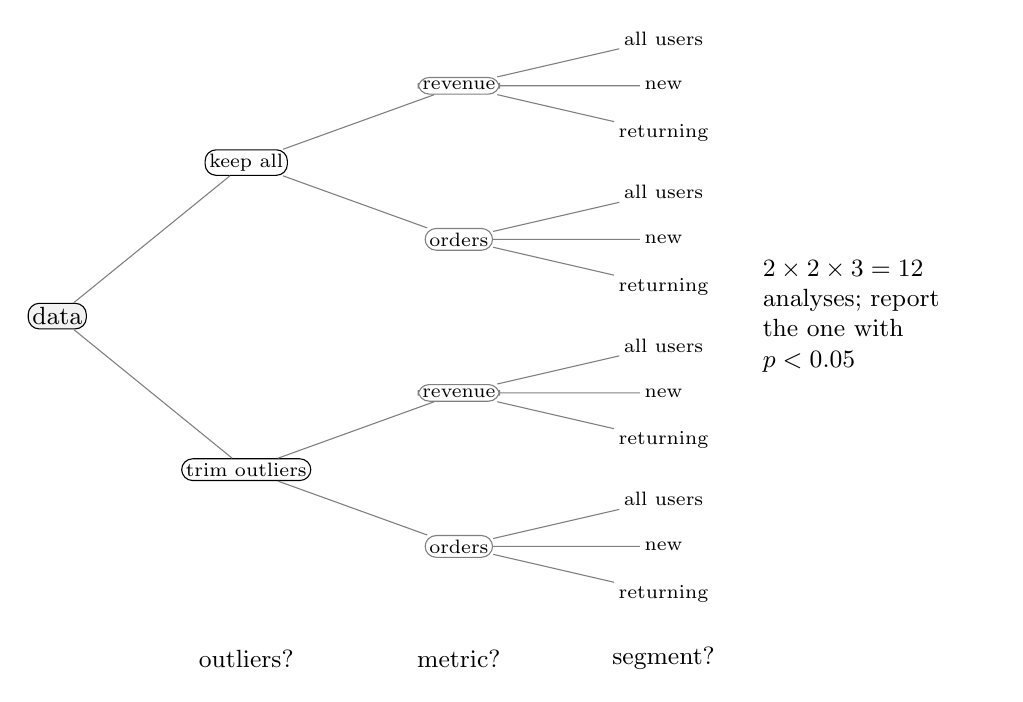
\begin{tikzpicture}[
  grow=right,
  level 1/.style={sibling distance=3.9cm, level distance=2.4cm},
  level 2/.style={sibling distance=1.95cm, level distance=2.7cm},
  level 3/.style={sibling distance=0.6cm, level distance=2.6cm},
  every node/.style={font=\scriptsize, inner sep=1.5pt},
  edge from parent/.style={draw, gray},
]
\node[draw, rounded corners, fill=gray!10, font=\small] {data}
  child { node[draw, rounded corners] {trim outliers}
    child { node[draw, rounded corners] {orders}
      child { node {returning} } child { node {new} } child { node {all users} } }
    child { node[draw, rounded corners] {revenue}
      child { node {returning} } child { node {new} } child { node {all users} } } }
  child { node[draw, rounded corners] {keep all}
    child { node[draw, rounded corners] {orders}
      child { node {returning} } child { node {new} } child { node {all users} } }
    child { node[draw, rounded corners] {revenue}
      child { node {returning} } child { node {new} } child { node {all users} } } };
\node[font=\small, align=center] at (2.4,-4.35) {outliers?};
\node[font=\small, align=center] at (5.1,-4.35) {metric?};
\node[font=\small, align=center] at (7.7,-4.35) {segment?};
\node[font=\small, align=left, anchor=west, text width=2.9cm] at (8.9,0) {$2\times2\times3=12$\\analyses; report\\the one with\\$p<0.05$};
\end{tikzpicture}
\caption{Three innocent-looking choices produce 12 different analyses of the same
A/B test. If the analyst picks a path after seeing which one ``works'', the effective
number of tests is 12, not 1.}
\label{fig:pitfalls-forks}
\end{figure}

If the 12 analyses were independent, the chance that at least one gives $p<0.05$
under a true null would be $1-0.95^{12}\approx 0.46$. They are not independent,
since they reuse the same users, so the true rate is lower. A simulation
answers the question. Generate 2000 fake A/B tests with 2000 users per arm and
\emph{no} real difference, run all 12 analyses on each, and count how often the best
one is ``significant''. Depending on how strongly the analyses overlap, the answer
comes out at roughly $25$ to $35\%$, five or more times the advertised $5\%$, even
though each single analysis taken alone fires about $5\%$ of the time.

The cure is to fix the analysis before seeing the outcome. A
\textbf{pre-registration} is a dated, written plan that names the primary metric,
the population, the exclusion rules and the test. Anything else you then look at
is labelled exploratory: interesting, but a hypothesis for the next experiment,
not a conclusion.

\subsection{Optional stopping: the peeking problem}

The most common fork in industry is time. A product manager checks the A/B
dashboard every morning and stops the test the first day it shows $p<0.05$.

Here is what that does. Take an A/A test, where both arms are identical so every
``win'' is false. Plan for 1000 observations. At each peek compute the $z$
statistic on all data so far and stop if $|z|>1.96$.
Figure~\ref{fig:pitfalls-path} follows one such test, peeking every 10
observations.

\begin{figure}[H]
\centering
\begin{tikzpicture}
\begin{axis}[
  width=12cm, height=6cm,
  xmin=0, xmax=1000, ymin=-2.6, ymax=2.6,
  xlabel={observations so far},
  ylabel={$z$ statistic},
  axis lines=left, grid=major, grid style={gray!20},
  title={One A/A test (no true difference), $z$ recomputed every 10 observations},
  title style={font=\small},
]
\fill[trapred!10] (axis cs:0,1.96) rectangle (axis cs:1000,2.6);
\fill[trapred!10] (axis cs:0,-2.6) rectangle (axis cs:1000,-1.96);
\draw[trapred, dashed] (axis cs:0,1.96) -- (axis cs:1000,1.96);
\draw[trapred, dashed] (axis cs:0,-1.96) -- (axis cs:1000,-1.96);
\node[trapred, font=\small, anchor=north west] at (axis cs:10,-2.0) {``significant'' zone $|z|>1.96$};
\addplot[distblue, thick] coordinates {
(10,-0.49) (20,-0.47) (30,0.55) (40,0.38) (50,0.73) (60,1.04) (70,0.84) (80,0.69) (90,0.89) (100,1.19) (110,1.47) (120,1.24) (130,1.24) (140,1.20) (150,0.85) (160,0.49) (170,0.63) (180,0.85) (190,1.15) (200,0.83) (210,0.80) (220,0.69) (230,0.51) (240,0.49) (250,0.52) (260,0.33) (270,0.48) (280,0.11) (290,0.35) (300,0.50) (310,0.41) (320,0.32) (330,0.37) (340,0.23) (350,0.27) (360,0.20) (370,0.40) (380,0.35) (390,0.29) (400,0.53) (410,0.84) (420,1.00) (430,0.80) (440,0.95) (450,0.92) (460,0.75) (470,0.84) (480,0.78) (490,0.82) (500,0.73) (510,0.66) (520,0.65) (530,0.49) (540,0.76) (550,0.97) (560,1.15) (570,1.18) (580,1.07) (590,1.13) (600,1.26) (610,1.30) (620,1.14) (630,1.36) (640,1.57) (650,1.61) (660,1.49) (670,1.54) (680,1.54) (690,1.75) (700,2.03) (710,2.09) (720,2.03) (730,1.98) (740,1.64) (750,1.87) (760,1.77) (770,1.68) (780,1.41) (790,1.26) (800,1.21) (810,1.10) (820,1.11) (830,1.23) (840,1.22) (850,1.02) (860,1.13) (870,1.06) (880,1.07) (890,1.13) (900,0.98) (910,1.04) (920,0.96) (930,0.88) (940,0.89) (950,0.83) (960,0.81) (970,0.94) (980,0.77) (990,0.68) (1000,0.61)
};
\fill[trapred] (axis cs:700,2.03) circle (2.4pt);
\node[font=\small, anchor=south east, fill=white, inner sep=1pt] at (axis cs:690,2.12) {peeker stops here and ships};
\fill[black] (axis cs:1000,0.61) circle (2.4pt);
\node[font=\small, anchor=north east] at (axis cs:995,0.5) {planned end: $z=0.61$};
\end{axis}
\end{tikzpicture}
\caption{A real path from the simulation below. The $z$ statistic wanders like a
random walk. It pokes into the red zone at $n=700$, and a daily peeker declares
victory. Had the test run to its planned end it would have shown nothing.}
\label{fig:pitfalls-path}
\end{figure}

Each single look has a 5\% false-positive rate. But you get many looks at a
wandering path, and you stop at whichever one is extreme. Simulating 20{,}000
A/A tests with equally spaced peeks shows how bad it gets. Figure~\ref{fig:pitfalls-peeking} shows the share
of A/A tests that were ever declared significant.

\begin{figure}[H]
\centering
\begin{tikzpicture}
\begin{axis}[
  width=11.5cm, height=6.2cm,
  xmode=log, xmin=0.8, xmax=1300,
  ymin=0, ymax=0.6,
  xtick={1,2,5,10,20,50,100,200,500,1000},
  xticklabels={1,2,5,10,20,50,100,200,500,1000},
  yticklabel style={/pgf/number format/fixed},
  xlabel={number of peeks (equally spaced over 1000 observations)},
  ylabel={false positive rate},
  axis lines=left, grid=major, grid style={gray!20},
  title={20{,}000 simulated A/A tests, stop at first $|z|>1.96$},
  title style={font=\small},
]
\addplot[trapred, very thick, mark=*, mark size=2pt] coordinates {
(1,0.0484) (2,0.0804) (3,0.1056) (5,0.1388) (10,0.1918) (20,0.2483) (50,0.3228) (100,0.3771) (200,0.4294) (500,0.4892) (1000,0.5318)};
\draw[targetgreen, dashed, thick] (axis cs:0.8,0.05) -- (axis cs:1300,0.05);
\node[targetgreen, font=\small, anchor=south east] at (axis cs:1250,0.055) {nominal $5\%$};
\node[font=\small, anchor=north west] at (axis cs:5,0.13) {5 peeks: $13.9\%$};
\node[font=\small, anchor=south east] at (axis cs:95,0.39) {100 peeks: $37.7\%$};
\end{axis}
\end{tikzpicture}
\caption{False positive rate of ``stop when significant'' as a function of how often
you look. Five looks nearly triple the error rate. Checking after every observation
pushes it past $50\%$. With unlimited patience it would reach $100\%$: the $z$
statistic of a never-ending A/A test eventually crosses any fixed threshold (the law
of the iterated logarithm).}
\label{fig:pitfalls-peeking}
\end{figure}

\begin{lstlisting}[language=Python]
import numpy as np
rng = np.random.default_rng(11)
R, N = 20000, 1000
S = np.cumsum(rng.standard_normal((R, N)), axis=1)  # A/A: true effect 0
for k in [1, 5, 20, 100]:
    looks = np.arange(1, k+1) * N // k
    z = S[:, looks-1] / np.sqrt(looks)
    print(k, (np.abs(z) > 1.96).any(axis=1).mean())  # .048 .139 .248 .377
\end{lstlisting}

\subsection{Sequential testing: peeking done right}

Peeking is not wrong in itself. Stopping a clearly harmful test early is good
practice. The problem is using a $1.96$ threshold at every look. A
\textbf{sequential test} plans the looks in advance and uses stricter thresholds so
that the total false-positive rate across all looks stays at $\alpha$.

\begin{itemize}
\item \textbf{Pocock boundary}: the same stricter threshold at every look. For 5
  equally spaced looks it is $|z|>2.41$. In the same 20{,}000 simulated A/A tests,
  this gives a $4.9\%$ false positive rate.
\item \textbf{O'Brien--Fleming boundary}: very strict early, close to $1.96$ at the
  end. For 5 looks the thresholds are $4.56,\ 3.23,\ 2.63,\ 2.28,\ 2.04$. Early
  stops need overwhelming evidence, and the final look costs almost nothing.
  Simulated rate: $4.9\%$.
\item \textbf{Always-valid methods} (mixture sequential probability ratio tests,
  ``anytime p-values'') let you look after every observation. Many commercial A/B
  platforms use them.
\end{itemize}

The general idea is called \textbf{alpha spending}: you have a budget of $0.05$
false-positive probability, and each look spends part of it. You can look as often
as you like, provided the thresholds were set to respect the budget before the
data arrived.

\section{Publication bias and the winner's curse}
\label{sec:pitfalls-winner}

Now zoom out from one analyst to a whole field. Journals, conference talks and
launch reviews favour significant results. Studies with $p>0.05$ end up in a
drawer. This is \textbf{publication bias}, and it distorts the published record
even if every individual study is honest.

Take a concrete case. A feature truly lifts a metric by 1 unit. Experiments are
underpowered: each estimate has standard error 1, so the estimate
$\hat\theta\sim\Normal(1,1)$. A result gets published (or launched) only if it is
significant in the positive direction, $\hat\theta>1.96$.

\begin{figure}[H]
\centering
\begin{tikzpicture}
\begin{axis}[
  width=12cm, height=6cm,
  domain=-2.5:4.5, samples=140,
  xmin=-2.5, xmax=4.5, ymin=0, ymax=0.48,
  xlabel={estimated effect $\hat\theta$},
  ylabel={density},
  axis lines=left, ytick=\empty,
  xtick={-2,-1,0,1,1.96,3,4},
  xticklabels={$-2$,$-1$,$0$,$1$,$1.96$,$3$,$4$},
  title={All experiments versus the ones that get published},
  title style={font=\small},
  clip=false,
]
\addplot[name path=curve, distblue, very thick] {0.3989*exp(-(x-1)^2/2)};
\path[name path=axisline] (axis cs:-2.5,0) -- (axis cs:4.5,0);
\addplot[densityred, fill opacity=0.35] fill between[of=curve and axisline, soft clip={domain=1.96:4.5}];
\draw[black, thick] (axis cs:1,0) -- (axis cs:1,0.42);
\node[font=\small, anchor=south] at (axis cs:1,0.42) {true effect $1.0$};
\draw[densityred, thick, dashed] (axis cs:2.49,0) -- (axis cs:2.49,0.30);
\node[font=\small, densityred, anchor=south west] at (axis cs:2.3,0.30) {mean published $2.49$};
\draw[gray, thick] (axis cs:1.96,0) -- (axis cs:1.96,0.12);
\node[font=\small, densityred, anchor=west] at (axis cs:3.1,0.08) {published: $17\%$};
\end{axis}
\end{tikzpicture}
\caption{Every experiment's estimate is drawn from the blue curve, centred on the
truth. Only the red tail clears the significance bar. The published estimates
average $2.49$, two and a half times the true effect, and every one of them
overstates the truth by at least $0.96$.}
\label{fig:pitfalls-winner}
\end{figure}

The share that clears the bar is the power: $P(\hat\theta>1.96)=P(Z>0.96)\approx
0.17$. The average published estimate is the mean of a Normal tail, which has a
closed form:
\[
  \E[\hat\theta \mid \hat\theta>1.96] = 1+\frac{\varphi(0.96)}{1-\Phi(0.96)}
  = 1+\frac{0.2516}{0.1685}\approx 2.49 .
\]
Here $\varphi$ is the standard Normal density (the height of the bell curve) and
$\Phi$ its CDF (the area to the left of a point).

This is the \textbf{winner's curse}: an estimate selected \emph{because} it was
large is biased upward. It bites at every scale. Among 20 launched features,
the ones whose A/B tests looked best will usually disappoint when measured again.
Lower power makes the curse stronger, because only wild overestimates can clear
the bar.

\begin{trapbox}
If a follow-up study finds a smaller effect than the original, the usual reason is
not that the effect ``decayed''. The original estimate was inflated by selection.
Plan follow-up sample sizes using a shrunken estimate, not the headline number.
\end{trapbox}

\section{Regression to the mean}
\label{sec:pitfalls-rtm}

A school gives 120 students two equally hard tests a week apart. The 15 best
scorers on test 1 (scores of 81 or more) averaged $84.9$. On test 2 the same
students averaged $76.9$. The 16 worst on test 1 (58 or less) averaged $54.9$
and then $60.7$. A tutoring programme for the bottom group would look like a
success, and praise for the top group like a disaster. Neither did anything.

\begin{figure}[H]
\centering
\begin{tikzpicture}
\begin{axis}[
  width=8.6cm, height=8.6cm,
  xmin=45, xmax=95, ymin=45, ymax=95,
  xlabel={test 1 score}, ylabel={test 2 score},
  axis lines=left, grid=major, grid style={gray!20},
  legend style={font=\scriptsize, at={(1.03,0.5)}, anchor=west},
  title={120 students, same skill, two noisy tests},
  title style={font=\small},
]
\addplot[only marks, mark=*, mark size=1.4pt, gray!60] coordinates {
(75,63) (70,70) (72,77) (73,78) (65,63) (65,61) (66,68) (73,77) (77,62) (62,61) (68,60) (75,70) (67,58) (73,71) (61,66) (69,71) (61,74) (62,69) (79,72) (73,69) (75,68) (73,71) (68,80) (69,64) (75,63) (77,76) (60,60) (59,74) (67,62) (65,78) (71,66) (62,66) (60,59) (70,71) (67,73) (71,56) (66,74) (80,68) (69,56) (60,64) (79,86) (78,71) (74,82) (76,70) (78,65) (66,65) (75,77) (66,77) (66,69) (75,81) (70,80) (75,68) (74,65) (66,64) (66,55) (79,73) (71,55) (60,52) (71,62) (76,59) (59,74) (70,77) (62,64) (67,70) (69,78) (64,61) (72,60) (66,70) (65,62) (80,65) (71,66) (62,58) (62,61) (68,60) (67,66) (67,83) (66,67) (66,73) (65,74) (79,76) (75,59) (70,69) (61,65) (69,66) (63,62) (59,60) (75,68) (66,65) (69,76)};
\addlegendentry{students}
\addplot[only marks, mark=*, mark size=1.8pt, distblue] coordinates {
(83,78) (86,81) (81,73) (82,83) (83,72) (81,72) (89,80) (88,84) (83,70) (91,76) (81,71) (92,83) (89,76) (84,77) (81,78)};
\addlegendentry{top 15 on test 1}
\addplot[only marks, mark=*, mark size=1.8pt, densityred] coordinates {
(52,67) (56,52) (57,60) (56,59) (58,54) (54,62) (50,52) (58,66) (55,66) (53,62) (52,63) (48,67) (58,55) (58,63) (56,64) (58,59)};
\addlegendentry{bottom 16 on test 1}
\addplot[black, dashed, domain=45:95] {x};
\addlegendentry{$y=x$ (no change)}
\addplot[structurepurple, very thick, domain=45:95] {35.28+0.4738*x};
\addlegendentry{fitted line, slope $0.47$}
\fill[distblue] (axis cs:84.9,76.9) circle (3.5pt);
\fill[densityred] (axis cs:54.9,60.7) circle (3.5pt);
\end{axis}
\end{tikzpicture}
\caption{Simulated scores: each student has a fixed skill, and each test adds
independent noise. Blue points (top on test 1) sit mostly \emph{below} the
diagonal, red points (bottom on test 1) mostly \emph{above}. The fitted line is
flatter than $y=x$. Extremes on the first measurement are partly luck, and luck
does not repeat. The two large dots are the group means.}
\label{fig:pitfalls-rtm}
\end{figure}

\begin{whybox}
Write each score as skill plus noise: $X_1=S+\eps_1$, $X_2=S+\eps_2$, with the noises
independent of each other and of skill. A student who scored very high on test 1
probably has high skill \emph{and} a lucky $\eps_1$. On test 2 the skill carries
over and the luck is redrawn with mean zero. So the expected second score is pulled
back toward the average. In the simulation, skill had SD 8 and each noise SD 6, so
the theoretical slope is
\[
  \frac{\Var(S)}{\Var(S)+\Var(\eps)}=\frac{64}{64+36}=0.64 .
\]
A slope below 1 is exactly ``regression toward the mean''. (This sample of 120
happens to give $0.47$, on the low side: a slope fitted to 120 noisy points still
wobbles by about $\pm0.07$ from sample to sample.) Chapter 12 shows that the least-squares slope
always equals $r\,s_y/s_x$, and with equal spreads that is just the correlation
$r<1$.
\end{whybox}

Regression to the mean fools people whenever units are \emph{selected because they
were extreme}: the worst-performing stores get a new manager, patients enrol in a
trial when symptoms peak, the rookie of the year has a ``sophomore slump''. The
defence is a control group selected the same way. Compare treated extreme units with
untreated extreme units, and the regression effect cancels.

\section{Base rates: how many significant findings are true?}
\label{sec:pitfalls-ppv}

A p-value below $0.05$ does \emph{not} mean a 95\% chance the effect is real. The
chance depends on how many of the hypotheses you test were real to begin with. Take
1000 ideas tested by a product team. Suppose 10\% truly work, the tests have 80\%
power, and $\alpha=0.05$.

\begin{figure}[H]
\centering
\begin{tikzpicture}[
  every node/.style={draw, rounded corners, align=center, font=\small, minimum width=2.3cm},
  level 1/.style={sibling distance=6.2cm, level distance=1.9cm},
  level 2/.style={sibling distance=3.0cm, level distance=2.1cm},
  edge from parent/.style={draw, -{Stealth}, gray!70!black},
  lab/.style={draw=none, font=\scriptsize, fill=white, inner sep=1pt, minimum width=0pt},
]
\node[fill=gray!10] {1000 ideas tested}
  child { node[fill=targetgreen!15] {100 really work}
    child { node[fill=targetgreen!35] {80 significant\\(true positives)} edge from parent node[lab, left] {power $0.8$} }
    child { node {20 missed} edge from parent node[lab, right] {$0.2$} }
    edge from parent node[lab, above left] {prior $10\%$} }
  child { node[fill=trapred!10] {900 do nothing}
    child { node[fill=trapred!30] {45 significant\\(false positives)} edge from parent node[lab, left] {$\alpha=0.05$} }
    child { node {855 correctly\\not significant} edge from parent node[lab, right] {$0.95$} }
    edge from parent node[lab, above right] {$90\%$} };
\end{tikzpicture}
\caption{Of the $80+45=125$ significant results, only 80 are real. The chance that
a significant finding is true is $80/125=64\%$, not $95\%$. The 45 false positives
come from the large pool of ideas that do nothing.}
\label{fig:pitfalls-tree}
\end{figure}

\begin{definition}[Positive predictive value]
The \textbf{positive predictive value} (PPV) is the probability that a significant
result reflects a real effect. With prior share $\pi$ of real effects, power
$1-\beta$ and level $\alpha$, Bayes' rule gives
\[
  \mathrm{PPV}=\frac{(1-\beta)\,\pi}{(1-\beta)\,\pi+\alpha\,(1-\pi)} .
\]
\end{definition}

With $\pi=0.1$ and power $0.8$ this is $0.08/(0.08+0.045)=0.64$. Cut the power to
$0.2$, common in small studies, and it drops to $0.02/(0.02+0.045)\approx 0.31$:
most significant findings are false. This is the arithmetic behind John Ioannidis's
2005 paper ``Why most published research findings are false''. It is the same
base-rate effect that makes a positive test for a rare disease usually a false
alarm (see Probability From the Ground Up, the chapter on Bayes' rule).

\begin{figure}[H]
\centering
\begin{tikzpicture}
\begin{axis}[
  width=11cm, height=6.2cm,
  domain=0.005:0.6, samples=120,
  xmin=0, xmax=0.6, ymin=0, ymax=1,
  xlabel={prior share of real effects $\pi$},
  ylabel={PPV},
  axis lines=left, grid=major, grid style={gray!20},
  legend style={font=\small, at={(0.97,0.03)}, anchor=south east},
  title={How believable is a significant result? ($\alpha=0.05$)},
  title style={font=\small},
]
\addplot[distblue, very thick] {0.8*x/(0.8*x+0.05*(1-x))};
\addlegendentry{power $0.8$}
\addplot[trapred, very thick] {0.2*x/(0.2*x+0.05*(1-x))};
\addlegendentry{power $0.2$}
\fill[distblue] (axis cs:0.1,0.64) circle (2.2pt);
\node[font=\small, anchor=west] at (axis cs:0.115,0.6) {$0.64$};
\fill[trapred] (axis cs:0.1,0.3077) circle (2.2pt);
\node[font=\small, anchor=west] at (axis cs:0.115,0.27) {$0.31$};
\draw[gray, dashed] (axis cs:0.1,0) -- (axis cs:0.1,1);
\end{axis}
\end{tikzpicture}
\caption{The share of significant results that are real, as a function of how
plausible the tested ideas were to start with. Long-shot hypotheses tested with low
power produce mostly false positives, however small the p-values look.}
\label{fig:pitfalls-ppv}
\end{figure}

\begin{connectionbox}
In machine learning the same logic applies to leaderboards. If hundreds of model
variants are tried against one test set and the best is reported, its score has a
winner's curse and a multiple-testing problem at once. Held-out test sets that are
touched once, and fresh evaluation data for the final claim, are the field's
version of pre-registration (Chapter 15).
\end{connectionbox}

\section{Simpson's paradox, revisited}
\label{sec:pitfalls-simpson}

Chapter 4 met Simpson's paradox as a curiosity about correlation. It is also a
pitfall for effect sizes. The classic data are a 1986 comparison of two kidney
stone treatments.

\begin{center}
\begin{tabular}{lccc}
\toprule
 & Small stones & Large stones & All patients \\
\midrule
Treatment A & 81/87 $= 93\%$ & 192/263 $= 73\%$ & 273/350 $= 78\%$ \\
Treatment B & 234/270 $= 87\%$ & 55/80 $= 69\%$ & 289/350 $= 83\%$ \\
\bottomrule
\end{tabular}
\end{center}

\begin{figure}[H]
\centering
\begin{tikzpicture}
\begin{axis}[
  width=10.5cm, height=6cm,
  ybar, bar width=0.6cm,
  ymin=50, ymax=105, xmin=0.4, xmax=3.6,
  xtick={1,2,3}, xticklabels={small stones, large stones, all patients},
  ylabel={success rate (\%)},
  axis lines=left,
  nodes near coords, nodes near coords style={font=\scriptsize},
  legend style={font=\small, at={(1.02,0.5)}, anchor=west},
  title={Treatment A wins in each group but loses overall},
  title style={font=\small},
]
\addplot[fill=distblue!60, draw=distblue] coordinates {(1,93) (2,73) (3,78)};
\addlegendentry{A}
\addplot[fill=quotientorange!60, draw=quotientorange] coordinates {(1,87) (2,69) (3,83)};
\addlegendentry{B}
\end{axis}
\end{tikzpicture}
\caption{A beats B for small stones and for large stones, yet B looks better
overall. Doctors gave A mostly to the hard large-stone cases (263 of 350), so A's
overall rate is dragged down by case mix, not by the treatment.}
\label{fig:pitfalls-simpson}
\end{figure}

A pooled effect size averages over a mix of groups. If the mix differs between the
arms, the pooled comparison measures the mix as much as the treatment. Randomization
(Chapter 5) makes the mix equal in expectation, which is the main reason randomized
experiments are trusted. In observational data, compare within strata of the
confounder, or adjust for it with regression (Chapter 13).

\begin{trapbox}
Splitting the data is not automatically right either. If the splitting variable is
\emph{caused by} the treatment (say, ``patients who finished the course''), the
within-group comparison is the biased one. Which table to trust is a question about
causes, not arithmetic.
\end{trapbox}

\section{Survivorship bias}
\label{sec:pitfalls-survivor}

During the Second World War, analysts studied bombers returning from missions and
mapped where they had bullet holes, planning to armour those spots. The statistician
Abraham Wald pointed out that the sample contained only planes that came back. Holes in
the engines were rare among survivors because planes hit in the engines did not
return. The armour belonged where the holes were \emph{not}.

\textbf{Survivorship bias} is what you get when the data only include units that
passed some filter linked to the outcome. Mutual funds are the textbook case.
Figure~\ref{fig:pitfalls-funds} simulates 20 funds whose yearly returns are pure
noise: mean $0\%$, SD $15\%$. A fund is closed and dropped from the database when
its value falls below $80\%$ of the start.

\begin{figure}[H]
\centering
\begin{tikzpicture}
\begin{axis}[
  width=10.5cm, height=6.5cm,
  xmin=0, xmax=10, ymin=0.5, ymax=2.9, clip=false,
  xlabel={year}, ylabel={value of \$1 invested},
  axis lines=left, grid=major, grid style={gray!20},
  title={20 funds with zero expected return},
  title style={font=\small},
  legend style={font=\small, at={(0.02,0.98)}, anchor=north west},
]
\addlegendimage{targetgreen, thick}\addlegendentry{survived 10 years (8)}
\addlegendimage{gray!60, thick}\addlegendentry{closed, dropped from database (12)}
\addplot[gray!60, thick, forget plot] coordinates {(0,1.000) (1,1.306) (2,0.805) (3,0.856) (4,0.783)};
\addplot[gray!60, thick, forget plot] coordinates {(0,1.000) (1,1.034) (2,0.979) (3,0.938) (4,0.844) (5,0.710)};
\addplot[gray!60, thick, forget plot] coordinates {(0,1.000) (1,0.867) (2,0.829) (3,0.939) (4,1.021) (5,1.035) (6,1.139) (7,0.656)};
\addplot[gray!60, thick, forget plot] coordinates {(0,1.000) (1,0.969) (2,0.835) (3,0.908) (4,0.987) (5,0.955) (6,0.843) (7,0.872) (8,0.546)};
\addplot[gray!60, thick, forget plot] coordinates {(0,1.000) (1,0.754)};
\addplot[gray!60, thick, forget plot] coordinates {(0,1.000) (1,1.049) (2,0.953) (3,1.181) (4,0.970) (5,1.021) (6,0.861) (7,1.042) (8,1.039) (9,0.981) (10,0.728)};
\addplot[gray!60, thick, forget plot] coordinates {(0,1.000) (1,0.911) (2,0.867) (3,0.896) (4,0.973) (5,0.791)};
\addplot[gray!60, thick, forget plot] coordinates {(0,1.000) (1,1.225) (2,1.500) (3,1.041) (4,0.988) (5,0.898) (6,0.969) (7,0.638)};
\addplot[gray!60, thick, forget plot] coordinates {(0,1.000) (1,0.853) (2,0.751)};
\addplot[gray!60, thick, forget plot] coordinates {(0,1.000) (1,0.860) (2,0.923) (3,1.263) (4,1.217) (5,1.115) (6,0.919) (7,0.735)};
\addplot[gray!60, thick, forget plot] coordinates {(0,1.000) (1,1.050) (2,1.068) (3,1.090) (4,0.841) (5,0.783)};
\addplot[gray!60, thick, forget plot] coordinates {(0,1.000) (1,0.901) (2,1.042) (3,0.941) (4,0.806) (5,0.720)};
\addplot[targetgreen, thick, forget plot] coordinates {(0,1.000) (1,1.004) (2,1.236) (3,1.337) (4,1.236) (5,1.202) (6,1.300) (7,1.677) (8,1.609) (9,1.550) (10,1.783)};
\addplot[targetgreen, thick, forget plot] coordinates {(0,1.000) (1,1.041) (2,1.151) (3,1.074) (4,0.901) (5,0.904) (6,0.897) (7,1.086) (8,1.208) (9,1.243) (10,1.450)};
\addplot[targetgreen, thick, forget plot] coordinates {(0,1.000) (1,1.252) (2,1.394) (3,1.551) (4,1.816) (5,1.911) (6,1.728) (7,1.520) (8,1.338) (9,1.613) (10,1.260)};
\addplot[targetgreen, thick, forget plot] coordinates {(0,1.000) (1,0.952) (2,0.994) (3,0.958) (4,1.075) (5,0.947) (6,0.966) (7,0.950) (8,1.028) (9,1.062) (10,1.469)};
\addplot[targetgreen, thick, forget plot] coordinates {(0,1.000) (1,1.205) (2,1.010) (3,0.981) (4,0.862) (5,1.056) (6,1.160) (7,1.107) (8,1.032) (9,1.107) (10,0.990)};
\addplot[targetgreen, thick, forget plot] coordinates {(0,1.000) (1,1.128) (2,1.059) (3,1.035) (4,1.161) (5,1.273) (6,1.597) (7,1.096) (8,1.237) (9,1.148) (10,1.171)};
\addplot[targetgreen, thick, forget plot] coordinates {(0,1.000) (1,1.126) (2,1.309) (3,1.513) (4,1.548) (5,1.921) (6,1.840) (7,1.801) (8,2.017) (9,1.850) (10,2.450)};
\addplot[targetgreen, thick, forget plot] coordinates {(0,1.000) (1,1.153) (2,1.529) (3,1.523) (4,1.435) (5,1.471) (6,1.634) (7,1.490) (8,1.574) (9,1.571) (10,1.951)};
\draw[trapred, dashed] (axis cs:0,0.8) -- (axis cs:10,0.8);
\node[trapred, font=\small, anchor=west, align=left] at (axis cs:10.15,0.8) {closure\\[-2pt]line};
\end{axis}
\end{tikzpicture}
\caption{Every fund here has zero expected return; their paths are pure luck. The
12 grey funds hit the closure line and vanish from the database. The 8 green
survivors average $+4.2\%$ a year. A ``ten-year track record'' study of today's funds
sees only the green lines and concludes that fund managers beat the market.}
\label{fig:pitfalls-funds}
\end{figure}

Survivorship bias shows up as: startup advice drawn from successful founders;
``old buildings were built better'' (the badly built ones fell down); churn
analyses that look only at current customers; and model training sets built from
loans that were approved, so the model never sees the applicants who were turned
away. The question to ask is always: \emph{what filter decided which units I get
to see, and could that filter be related to the outcome?}

\section{A checklist for reading a statistical claim}
\label{sec:pitfalls-checklist}

Every pitfall in this chapter maps to one question. Run through them in order when
you read a paper, a dashboard or a launch memo.

\begin{figure}[H]
\centering
\begin{tikzpicture}[
  node distance=0.28cm,
  q/.style={draw, rounded corners, fill=distblue!8, text width=10.6cm, font=\small, inner sep=4pt, align=left},
]
\node[q] (a) {\textbf{1. How big?} Is there an effect size in real units, with a confidence interval? Is it bigger than the smallest effect that matters?};
\node[q, below=of a] (b) {\textbf{2. Compared with what?} What is the baseline? Are ratios given with absolute numbers?};
\node[q, below=of b] (c) {\textbf{3. How many tries?} How many metrics, subgroups, models or analyses were looked at? Was there a correction or a pre-registered primary metric?};
\node[q, below=of c] (d) {\textbf{4. When did they stop?} Fixed sample size, a proper sequential design, or ``until it was significant''?};
\node[q, below=of d] (e) {\textbf{5. Why am I seeing this?} Was it selected for being striking (publication bias, winner's curse, top performers)? Has it been replicated?};
\node[q, below=of e] (f) {\textbf{6. Selected for being extreme?} Could a before/after change be regression to the mean? Is there a control group?};
\node[q, below=of f] (g) {\textbf{7. How plausible beforehand?} Low prior plus low power means most significant results are false.};
\node[q, below=of g] (h) {\textbf{8. Who is missing?} Randomized, or could confounding (Simpson) or survivorship explain it?};
\end{tikzpicture}
\caption{Eight questions, one for each pitfall in this chapter. A claim that
survives all eight deserves to be taken seriously.}
\label{fig:pitfalls-checklist}
\end{figure}

\begin{walkbox}
Headline: ``Our new onboarding flow boosts 30-day retention by 35\% ($p=0.03$).''
Running the checklist: (1) 35\% relative lift on what base? From 2\% to 2.7\% is
0.7 points. Ask for the interval. (2) Which baseline cohort? (3) The memo shows 14
retention and engagement metrics; retention was the one that came out significant. With
14 tests the chance of at least one false positive is about 51\%. (4) The test ran
``until results stabilised'': that is optional stopping. (5) This is the one result of
several experiments that made it into the memo. Verdict: interesting, not
established. Rerun with retention as the pre-registered primary metric and a fixed
sample size.
\end{walkbox}

\section{Summary}
\label{sec:pitfalls-summary}

\begin{center}
\renewcommand{\arraystretch}{1.3}
\begin{tabular}{p{3.4cm}p{9.0cm}}
\toprule
Idea & Key fact \\
\midrule
Practical significance & Large $n$ makes tiny effects significant. Judge the CI against the smallest effect that matters. \\
Effect sizes & Difference in natural units with CI first; Cohen's $d$ for unitless scales; for rates give absolute difference and RR/OR together. \\
Report CIs & An interval contains the test result plus size and precision. \\
Multiple testing & $\mathrm{FWER}=1-(1-\alpha)^m$. Bonferroni ($\alpha/m$) and Holm control FWER; BH controls FDR via $p_{(k)}\le qk/m$. \\
Forking paths & Data-dependent analysis choices are hidden multiple tests. Pre-register. \\
Optional stopping & Stopping at first $p<0.05$ inflates false positives (14\% at 5 peeks, 38\% at 100). Use sequential boundaries. \\
Winner's curse & Estimates selected for significance are inflated, badly so at low power. \\
Regression to the mean & Units selected for being extreme drift back. Needs a control group. \\
PPV & $\mathrm{PPV}=\dfrac{(1-\beta)\pi}{(1-\beta)\pi+\alpha(1-\pi)}$; low prior and low power make most hits false. \\
Simpson, survivorship & Pooled comparisons and filtered samples can reverse or invent effects. \\
\bottomrule
\end{tabular}
\end{center}

Chapter 12 moves from comparing groups to modelling a relationship: the regression
line, whose slope below one you have already seen in the regression-to-the-mean
picture.

\section{Exercises}
\label{sec:pitfalls-exercises}

\begin{enumerate}
\item An A/B test with $n=200{,}000$ per arm finds conversion $5.00\%$ versus
  $5.05\%$. Compute the 95\% CI for the difference (unpooled SE). Is it
  significant? Would you ship if the smallest effect of interest is $0.2$ points?
\item Two groups of 30 have means $82$ and $76$ and SDs $10$ and $14$. Compute
  Cohen's $d$ with the pooled SD.
\item A drug raises the rate of a side effect from $30\%$ to $45\%$. Give the
  absolute difference, the risk ratio and the odds ratio. Which number would a
  headline writer prefer?
\item How many independent tests at $\alpha=0.05$ make the chance of at least one
  false positive exceed $90\%$?
\item Apply Bonferroni, Holm and BH ($q=0.05$) to the six p-values
  $0.002$, $0.009$, $0.012$, $0.030$, $0.041$, $0.380$. How many does each reject?
\item In the peeking simulation, the false positive rate with 5 peeks was about
  $14\%$. Explain in two sentences why it is not $1-0.95^5\approx 23\%$.
\item A field tests hypotheses of which $5\%$ are true, with power $0.5$ and
  $\alpha=0.05$. What fraction of significant findings are true?
\item A city installs speed cameras at the 10 junctions with the most crashes last
  year. Next year crashes there fall by 30\%. Give a reason to doubt that the cameras
  caused all of it, and describe a better comparison.
\item An article reports that the average customer who has stayed 5 years spends
  more per month than new customers, and concludes that customers spend more the
  longer they stay. Name the bias and explain.
\end{enumerate}

\subsection*{Answers}

\begin{enumerate}
\item Difference $0.05$ points; $\SE=\sqrt{0.05\cdot0.95/2\times10^{5}+0.0505\cdot0.9495/2\times10^{5}}\approx0.000691$,
  so CI $\approx 0.05\pm0.135=[-0.085,\ 0.185]$ points. Not significant
  ($z\approx0.72$). The whole interval lies below $0.2$, so even the most
  optimistic plausible lift is too small: do not ship. This is case (c), informative.
\item $s_p=\sqrt{(29\cdot100+29\cdot196)/58}=\sqrt{148}\approx12.17$, so
  $d=6/12.17\approx0.49$.
\item Difference $15$ points; $\mathrm{RR}=1.5$;
  $\mathrm{OR}=(0.45/0.55)/(0.30/0.70)\approx1.91$. The headline writer prefers the
  OR (``nearly doubles the odds''), which is easily misread as ``nearly twice as likely''.
\item $1-0.95^m>0.9$ means $m>\ln 0.1/\ln 0.95\approx 44.9$, so $m=45$.
\item Bonferroni ($0.05/6\approx0.00833$): rejects $0.002$ only, so 1.
  Holm: $0.002\le0.00833$, $0.009\le0.01$, $0.012\le0.0125$, then $0.030>0.01667$
  stops, so 3. BH thresholds are $0.00833$, $0.0167$, $0.025$, $0.0333$, $0.0417$,
  $0.05$; the last p-value under its threshold is $0.041\le0.0417$ at
  $k=5$, so 5 rejected.
\item The five looks share data: the $z$ at look 3 contains all the observations of
  looks 1 and 2, so the tests are strongly positively correlated. Correlated tests
  overlap in when they fire, so the union is smaller than the independent formula predicts.
\item $\mathrm{PPV}=0.5\cdot0.05/(0.5\cdot0.05+0.05\cdot0.95)=0.025/0.0725\approx0.34$.
\item Junctions were selected for an extreme year, so crashes would regress toward
  their long-run mean even with no cameras. Compare with similar high-crash junctions
  that did not get cameras (ideally chosen at random from the high-crash list), or
  use several years of history before selection.
\item Survivorship bias. Low-spending customers are more likely to churn, so the
  5-year group is filtered toward high spenders. Individual customers may not change
  their spending at all.
\end{enumerate}
